\section{Cronograma}
\label{sec:cronograma}

A Figura \ref{fig:cronograma} apresenta o cronograma do projeto.

\begin{figure}[H]
    \caption{Cronograma do projeto.}
    \label{fig:cronograma}
    \centering
    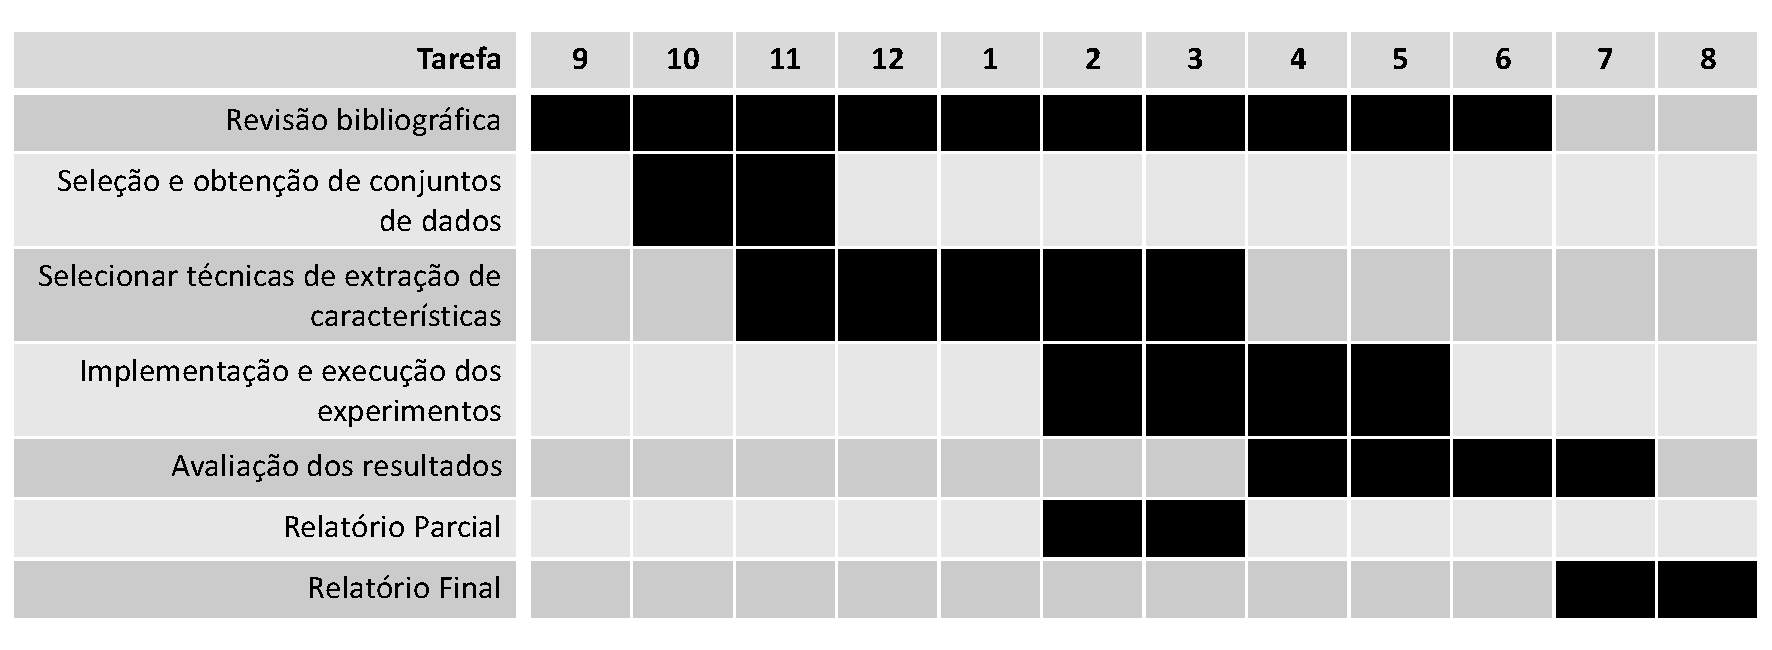
\includegraphics[width=\textwidth]{Cronograma.pdf}    
\end{figure}

As tarefas mencionadas no cronograma são brevemente descritas a seguir:

\begin{itemize}
    \item \textit{Revisão bibliográfica}: pesquisa de trabalhos relacionados a extração de características para biometria pela impressão digital;
    \item \textit{Seleção e obtenção de conjuntos de dados}: seleção de conjuntos de dados com imagens de impressão digital para serem utilizados nos experimentos. A Seção~\ref{sec:metodologia} menciona alguns conjuntos de dados que podem ser considerados;
    \item \textit{Selecionar técnicas de extração de características}: definir quais técnicas de extração de características para reconhecimento de usuários por impressão serão consideradas;    
    \item \textit{Implementação e execução dos experimentos}: implementação do código para avaliação das técnicas de extração de características e execução dos experimentos;
    \item \textit{Avaliação dos resultados}: avaliação dos resultados obtidos nos experimentos;
    \item \textit{Relatório Parcial}: elaboração do relatório parcial;
    \item \textit{Relatório Final}: elaboração do relatório final.
\end{itemize}